\chapter{Results and Evaluation} \label{Results and Evaluation}

In this chapter we analyze the performance of each of our trained models. We conduct a thorough performance evaluation and compare the results obtained with the RT-PCR test and a basic CNN. We also compare our results with related work highlighted in Section \ref{LR}. The heatmaps obtained have also been compared to the findings obtained by a professional Radiologist. 

% We have utilized the strategies proposed in Appendix \ref{Evaluation Strategy Section} for evaluation purposes.

\section{X-ray Scans}
The following sections evaluates results obtained by each of our X-ray models, followed by comparing them across various parameters.
% \vspace{-1em}
\subsection{Performance Evaluation}
We evaluate the performance of our three models, DenseNet121, ResNet50, and VGG16, across various metrics followed by showcasing the performance increase obtained by our Ensemble model. These sections are supplemented with tables, plots highlighting trends in loss and accuracy, and confusion matrices respectively. As we have performed 10-fold cross validation, we have obtained 10 confusion matrices whose values we have summed up to calculate average metric scores \cite{RGC2016}.
% \vspace{-1em}
\subsubsection{Pre-trained Models} \label{ptmXray}

The first model implemented is DenseNet121. Our 10-fold cross validation resulted in 94.6\% average accuracy on the balanced dataset. The average and best accuracy obtained on unseen data are 95.1\% and 96.8\% respectively. We have displayed classification report results indicating Precision, Recall, and F1-scores per class in Table \ref{tab:DenseNet CR} and confusion matrix in Figure \ref{fig:DenseNet121 Confusion Matrix},  followed by trends in accuracy and loss in Figure \ref{fig:densenetModelTraining}, of the best performing model.

\begin{table}[ht]
\begin{minipage}[b]{0.55\linewidth}
\centering
  \begin{longtable}{| p{.21\textwidth} |  p{.17\textwidth} |   p{.13\textwidth} | p{.11\textwidth} |} 
    \hline
& \textbf{Precision} & \textbf{Recall}    & \textbf{F1-Score}  \\
\hline
			COVID-19    &97.7\%   &97.7\%    &97.7\%
\\\hline
			Normal      &93.6\%   &92.7\%    &93.1\%
\\\hline 
            Pneumonia   &92.6\%       &93.5\%        &93.0\%
\\\hline

    \end{longtable}
        \vspace{0.5em}
    \begin{longtable}{| p{.52\textwidth} |  p{.13\textwidth}|} 
    \hline
    		\textbf{Accuracy}    &94.6\%
\\\hline
        \end{longtable}

    \vspace{1em}
 \captionsetup{width=.8\linewidth}
 \caption{DenseNet121 Classification Report}  \label{tab:DenseNet CR}
\end{minipage}
\begin{minipage}[b]{0.45\linewidth}
\centering
 \captionsetup{width=.8\linewidth}
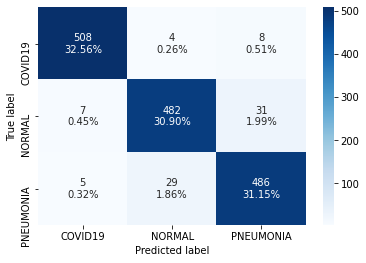
\includegraphics[width=\linewidth]{Images/DenseNetCM.png}
\captionof{figure}{DenseNet121 Confusion Matrix}
\label{fig:DenseNet121 Confusion Matrix}
\end{minipage}
\end{table}
\vspace{-\parskip}
\begin{figure}[H]
        \begin{subfigure}[b]{0.5\textwidth}
                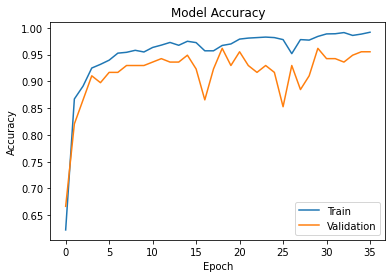
\includegraphics[width=\linewidth]{Images/DenseNetAccuracy.png}
        \end{subfigure}%
        \begin{subfigure}[b]{0.5\textwidth}
                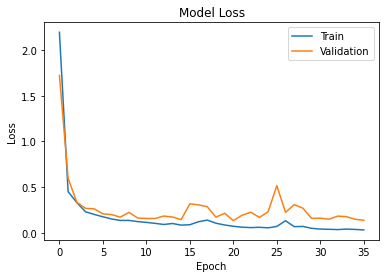
\includegraphics[width=\linewidth]{Images/DenseNetLoss.png}
        \end{subfigure}%
        %\\\centering
            %\decoRule
        \caption{DenseNet121 Model Training Performance Trends}\label{fig:densenetModelTraining}
\end{figure}
\vspace{-1em}
Next we have ResNet50 which is popular among literature as seen in Section \ref{LR}. We have achieved an average accuracy of 95.8\% after 10-fold cross validation on the balanced dataset. The average and best accuracy obtained on unseen data are 97.6\% and 98.1\% respectively. We have plotted the classification report, confusion matrix, and trends in accuracy and loss in Table \ref{tab:ResNet CR}, Figure \ref{fig:ResNet50 Confusion Matrix}, and Figure \ref{fig:resnetModelTraining} respectively.
    % \vspace{-1em}

\begin{table}[ht]
\begin{minipage}[b]{0.55\linewidth}
\centering

  \begin{longtable}{| p{.21\textwidth} |  p{.17\textwidth} |   p{.13\textwidth} | p{.11\textwidth} |} 
    \hline
& \textbf{Precision} & \textbf{Recall}    & \textbf{F1-Score}  \\
\hline
			COVID-19    &98.9\%   &99.0\%    &98.9\%
\\\hline
			Normal      &94.9\%   &93.3\%    &94.1\%
\\\hline 
            Pneumonia    &93.6\%   &95.0\%    &94.3\%
\\\hline

    \end{longtable}
        \vspace{0.5em}
    \begin{longtable}{| p{.52\textwidth} |  p{.13\textwidth}|} 
    \hline
    		\textbf{Accuracy}    &95.8\%
\\\hline
        \end{longtable}

    \vspace{1em}
     \captionsetup{width=.8\linewidth}

 \caption{ResNet50 Classification Report}  \label{tab:ResNet CR}
\end{minipage}
\begin{minipage}[b]{0.45\linewidth}
\centering
 \captionsetup{width=.8\linewidth}
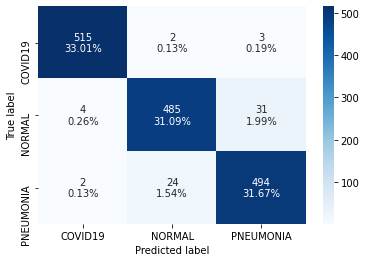
\includegraphics[width=1\linewidth]{Images/ResNetCM.png}


\captionof{figure}{ResNet50 Confusion Matrix}
\label{fig:ResNet50 Confusion Matrix}
\end{minipage}
\end{table}
\clearpage

\vspace{-\parskip}
\begin{figure}[H]
        \begin{subfigure}[b]{0.5\textwidth}
                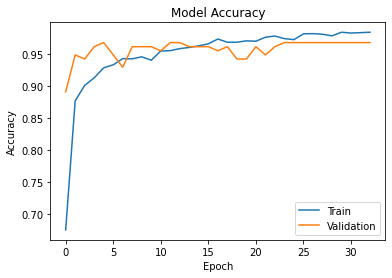
\includegraphics[width=\linewidth]{Images/ResNetAcc.png}
        \end{subfigure}%
        \begin{subfigure}[b]{0.5\textwidth}
                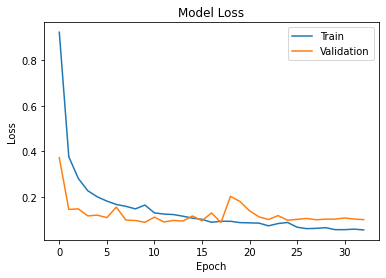
\includegraphics[width=\linewidth]{Images/ResNetLoss.png}
        \end{subfigure}%
        %\\\centering
            %\decoRule
        \caption{ResNet50 Model Training Performance Trends}\label{fig:resnetModelTraining}
\end{figure}
\vspace{-1em}
The final base model is VGG16. We have achieved an average accuracy of 95.6\% after 10-fold cross validation on the balanced dataset. The average and best accuracy obtained on unseen data are 95.3\% and 96.8\% respectively. The classification report, confusion matrix, and trends in accuracy and loss is displayed in Table \ref{tab:VGG CR}, Figure \ref{fig:VGG16 Confusion Matrix}, Figure \ref{fig:vggModelTraining}.

    % \vspace{1em}

\begin{table}[ht]
\begin{minipage}[b]{0.55\linewidth}
\centering
  \begin{longtable}{| p{.21\textwidth} |  p{.17\textwidth} |   p{.13\textwidth} | p{.11\textwidth} |} 
    \hline
& \textbf{Precision} & \textbf{Recall}    & \textbf{F1-Score}  \\
\hline
			COVID-19    &97.5\%   &98.9\%    &98.2\%
\\\hline
			Normal      &94.1\%   &94.6\%    &94.3\%
\\\hline 
            Pneumonia   &95.3\%       &93.5\%        &94.4\%
\\\hline

    \end{longtable}
        \vspace{0.5em}
    \begin{longtable}{| p{.52\textwidth} |  p{.13\textwidth}|} 
    \hline
    		\textbf{Accuracy}    &95.6\%
\\\hline
        \end{longtable}

    \vspace{1em}
     \captionsetup{width=.8\linewidth}

 \caption{VGG16 Classification Report}  \label{tab:VGG CR}
\end{minipage}
\begin{minipage}[b]{0.45\linewidth}
\centering
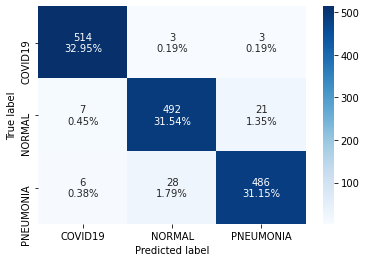
\includegraphics[width=1\linewidth]{Images/VGG16CM.png}
 \captionsetup{width=.7\linewidth}

\captionof{figure}{VGG16 Confusion Matrix}
\label{fig:VGG16 Confusion Matrix}
\end{minipage}
\end{table}


\begin{figure}[H]
        \begin{subfigure}[b]{0.5\textwidth}
                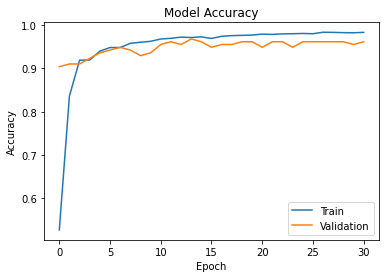
\includegraphics[width=\linewidth]{Images/VGGAcc.png}
        \end{subfigure}%
        \begin{subfigure}[b]{0.5\textwidth}
                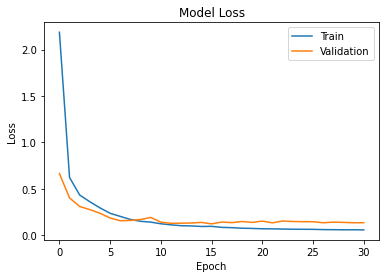
\includegraphics[width=\linewidth]{Images/VGGLoss.png}
        \end{subfigure}%
        %\\\centering
            %\decoRule
        \caption{VGG16 Model Training Performance Trends}\label{fig:vggModelTraining}
\end{figure}


\subsubsection{Ensemble Model}

After ensembling each of the three base models discussed in Section \ref{ptmXray}, we have evaluated the performance utilizing the classification report function, confusion matrix and trends in accuracy and loss. These are displayed in Table \ref{tab:EnsembleXray CR}, Figure \ref{fig:XRay Ensemble Confusion Matrix}, and Figure \ref{fig:xrayEnsembleModelTraining} respectively. We have achieved an average accuracy of 98.8\% after 10-fold cross validation on the balanced dataset. The average and best accuracy obtained on unseen data are 97.8\% and 98.1\% respectively.
    \vspace{1em}

\begin{table}[ht]
\begin{minipage}[b]{0.55\linewidth}
\centering
  \begin{longtable}{| p{.21\textwidth} |  p{.17\textwidth} |   p{.13\textwidth} | p{.11\textwidth} |} 
    \hline
& \textbf{Precision} & \textbf{Recall}    & \textbf{F1-Score}  \\
\hline
			COVID-19    &99.8\%   &99.8\%    &99.8\%
\\\hline
			Normal      &98.3\%   &98.5\%    &98.4\%
\\\hline 
            Pneumonia   &98.1\%       &98.3\%        &98.2\%
\\\hline

    \end{longtable}
        \vspace{0.5em}
    \begin{longtable}{| p{.52\textwidth} |  p{.13\textwidth}|} 
    \hline
    		\textbf{Accuracy}    &98.8\%
\\\hline
        \end{longtable}
 \captionsetup{width=.8\linewidth}
    \vspace{1em}
 \caption{X-ray Ensemble Model Classification Report}  \label{tab:EnsembleXray CR}
\end{minipage}
\begin{minipage}[b]{0.45\linewidth}
\centering
 \captionsetup{width=.8\linewidth}
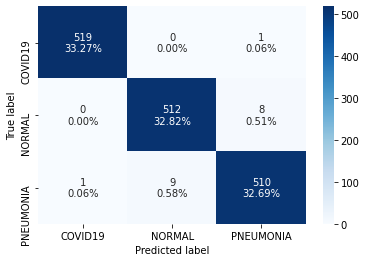
\includegraphics[width=1\linewidth]{Images/EnsembleXrayCM.png}
\captionof{figure}{X-ray Ensemble Model Confusion Matrix}
\label{fig:XRay Ensemble Confusion Matrix}
\end{minipage}
\end{table}


\begin{figure}[H]
        \begin{subfigure}[b]{0.5\textwidth}
                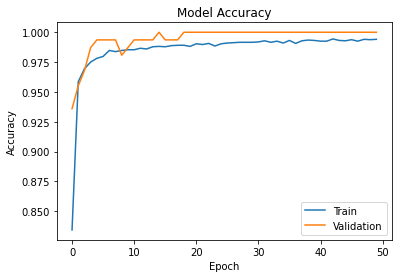
\includegraphics[width=\linewidth]{Images/EnsembleXrayAcc.png}
        \end{subfigure}%
        \begin{subfigure}[b]{0.5\textwidth}
                \includegraphics[width=\linewidth]{Images/EnsembleXrayLoss.png}
        \end{subfigure}%
        %\\\centering
            %\decoRule
        \caption{X-ray Ensemble Model Training Performance Trends}\label{fig:xrayEnsembleModelTraining}
\end{figure}


\subsection{Performance Comparison}
In the following sections we compare the performance of our models with respect to each other and determine the best performing model, followed by comparing the best results with that of the RT-PCR test and CNN. We also compare our results with related studies observed in the literature. We conclude this section by comparing our heatmap results with that of the findings obtained by a professional Radiologist who has volunteered to help us in this study.

\subsubsection{Trained Models}

We compare each of our base X-ray models along with the ensemble model across various parameters such as Accuracy, Precision, Recall, F1-Score, Specificity, and Sensitivity respectively. These metric scores are tabulated in Table \ref{tab:mpcXray}.

\vspace{1em}
 \begin{longtable}{| p{.23\textwidth} |  p{.1\textwidth} |   p{.1\textwidth} | p{.06\textwidth} | p{.095\textwidth} | p{.11\textwidth} | p{.11\textwidth} |} 
    \hline
& \textbf{Accuracy} & \textbf{Precision} & \textbf{Recall} & \textbf{F1-Score} & \textbf{Specificity} & \textbf{Sensitivity} \\
\hline
			DenseNet121    &94.6\%   &94.6\%    &94.6\%    &94.6\%   &97.3\%   &94.6\% 
\\\hline
			ResNet50    &95.8\%   &95.8\%    &95.8\%    &95.8\%   &97.9\%   &95.8\% 
\\\hline
			VGG16    &95.6\%   &95.6\%    &95.6\%    &95.6\%   &99.0\%   &97.8\% 
\\\hline
	        \textbf{Ensemble Model}    &\textbf{98.8\%}   &\textbf{98.7\%}    &\textbf{98.9\%}    &\textbf{98.8\%}   &\textbf{99.4\%}   &\textbf{98.9\%} 
\\\hline
 \caption{X-ray Models Performance Comparison}  \label{tab:mpcXray}

    \end{longtable}
\vspace{-1em}
We observe that out of the base models, DenseNet121 and ResNet50 have very comparable results with the former having a slight performance increase when compared to the latter. However, the Ensemble Model clearly outperforms each of our base models as expected.

\subsubsection{RT-PCR and CNN}

We compare the results given by our Ensemble model, only for the \textbf{COVID-19 class}, with the RT-PCR test according to the study conducted by the Infectious Diseases Society of America (IDSA) \cite{IDS2020}. We also did implement a CNN-based model to compare our model with deep learning models that use state of the art techniques.
Table \ref{tab:comp} summarizes the comparison and uses three metrics, namely sensitivity and specificity (relatively to the COVID-19 class) as well as accuracy. 

 \begin{longtable}{| p{.15\textwidth} | p{.11\textwidth} |  p{.11\textwidth} |   p{.11\textwidth} |} 
    \hline
& \textbf{Accuracy} & \textbf{Sensitivity} & \textbf{Specificity} \\
\hline

			RT-PCR      &-   &84.2\%    &98.9\%  
\\\hline
			CNN    &93.9\%   &85.2\%    &98.2\% 
\\\hline
			\textbf{Our Approach}   &\textbf{99.9\%}   &\textbf{99.8\%}    &\textbf{99.9\%} 
\\\hline
 \caption{Comparison with RT-PCR and CNN for X-ray scans}  \label{tab:comp}
    \end{longtable}
\vspace{-1em}
As expected, our Ensemble model performs significantly better when compared to a basic CNN model. More importantly, our approach also exhibits better sensitivity and specificity when compared to the traditional RT-PCR test.

\subsubsection{Related Work}

In this section, we compare the performance of the Ensemble model with similar studies found in literature. We shall compare the results obtained by our best performing model with the scores reported by studies discussed in Section \ref{LR}. Table \ref{tab:relWorkXray} tabulates these results.

\vspace{1em}
 \begin{longtable}{| p{.23\textwidth} |  p{.1\textwidth} |   p{.1\textwidth} | p{.06\textwidth} | p{.095\textwidth} | p{.11\textwidth} | p{.11\textwidth} |} 
    \hline
& \textbf{Accuracy} & \textbf{Precision} & \textbf{Recall} & \textbf{F1-Score} & \textbf{Specificity} & \textbf{Sensitivity} \\
\hline
Wang et al. \cite{LWA2020}   &83.5\%    &98.9\%     &91.0\%   &94.7\%    &99.5\%     &91.0\%
\\\hline

Ghoshal et al. \cite{GHT2020}   &92.9\%    &66.7\%     &85.7\%   &75.0\%    &99.4\%     &85.7\%
\\\hline
Zhang et al. \cite{ZXS+2020}   &96.0\%    &59.6\%     &96.0\%   &73.5\%    &70.7\%     &96.0\%
\\\hline
Narin et al. \cite{AKP2020}   &98.0\%    &76.5\%     &91.8\%   &83.5\%    &96.6\%     &91.8\%
\\\hline
\textbf{Ensemble Model}    &\textbf{98.8\%}   &\textbf{98.7\%}    &\textbf{98.9\%}    &\textbf{98.8\%}   &\textbf{99.4\%}   &\textbf{98.9\%} 
\\\hline
 \caption{Comparison with Related Work}  \label{tab:relWorkXray}

    \end{longtable}
\vspace{-2em}

Our X-ray Ensemble model outperforms the results obtained by other studies across all metrics. We believe that various approaches considered such as Data Augmentation, Transfer Learning, and Ensemble Learning have helped our models achieve optimal classification performance.
\vspace{-1em}

\subsubsection{Radiologist Findings} \label{rfxray}

To further verify that the heatmaps produced by the model are in conformance with the same observed characteristics, we have provided a subset of X-rays scans to a senior Radiologist \footnote{The authors thank Dr. G.R. Mahadevan (MD, IDCCM,D.Diab, Specialist in COVID-19) from Maya Nursing Home,Tamil Nadu for annotating the X-ray and CT images.} and have asked to highlight the critical regions and provide their diagnosis results. 

Table \ref{tab:radioFinding} compares the Radiologist's annotations and diagnosis with those produced by our model along with the heatmap result.
We can observe that the heatmaps are in direct compliance with the Radiologists’ findings. Precisely, visually, the heatmaps show that our predictive model highlights at least one or more of the critical regions identified by the Radiologist. Furthermore, all areas highlighted by the Radiologist are shades of either red of purple, but never blue.

We have also verified that the heatmaps we obtained correspond to the regions highlighted from studies conducted by Harmon et al. \cite{HSX+2020} and Li et al. \cite{LLL+2020}. The lower lung lobes seem to be the most affected in patients diagnosed with COVID-19, this correlates with the observations from Chung et al. \cite{CMA+2020} and therefore, provides additional validation that lung characteristics such as GGO’s, consolidations, and lesions are major contributing factors to COVID-19 detection.

% \vspace{1em}

\begin{longtable} { | c | c | c | }
    \hline
    \textbf{Original} & \textbf{Radiologist Finding} & \textbf{Heatmap} \\ \hline
    \begin{minipage}{.3\textwidth}
    \vspace{1em}
      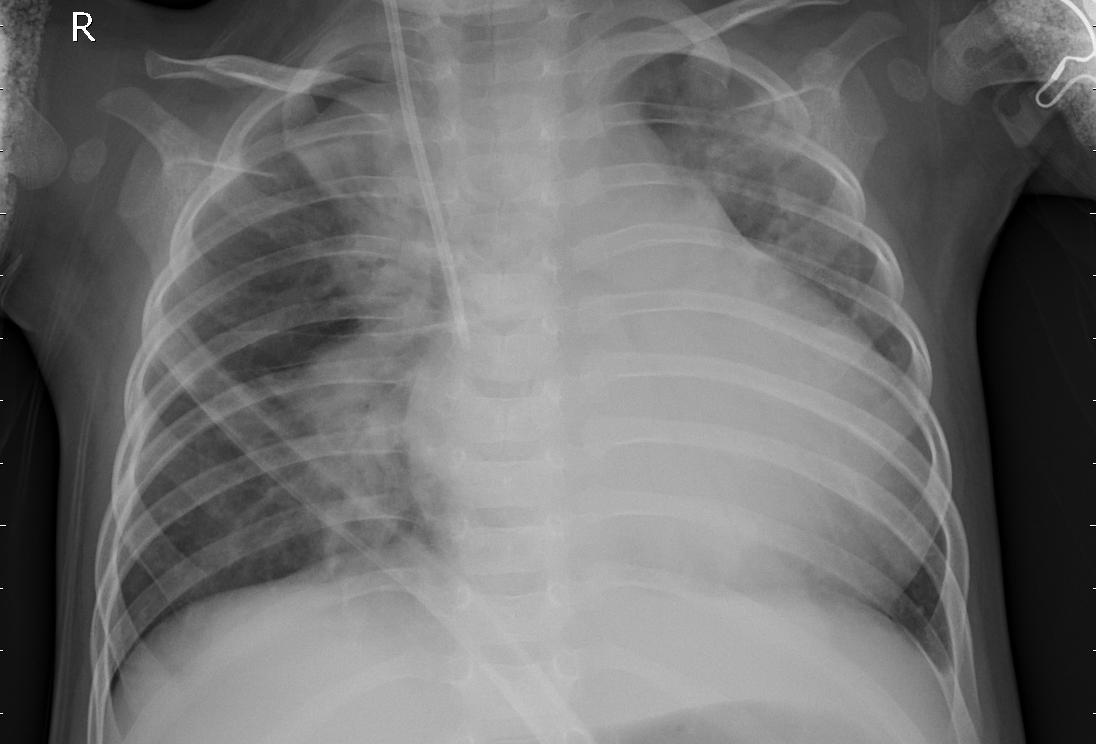
\includegraphics[width=\linewidth, height=30mm]{Images/PneumoniaOrig1.jpg}
    \vspace{0.5em}
    \end{minipage}
    &
  \begin{minipage}{.3\textwidth}
      \vspace{1em}
      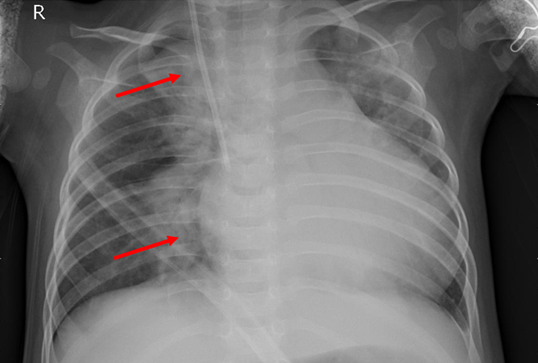
\includegraphics[width=\linewidth, height=30mm]{Images/PneuRadio1.png}
           \centering  Pneumonia
               \vspace{0.5em}
    \end{minipage}
    & 
    \begin{minipage}{.3\textwidth}
        \vspace{1em}
      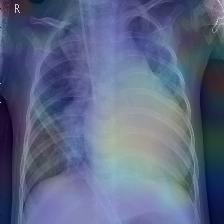
\includegraphics[width=\linewidth, height=30mm]{Images/PneumoniaHeatmap1.jpg}
      \centering Pneumonia
          \vspace{0.5em}
    \end{minipage}
    \\ \hline
        \begin{minipage}{.3\textwidth}
    \vspace{1em}
      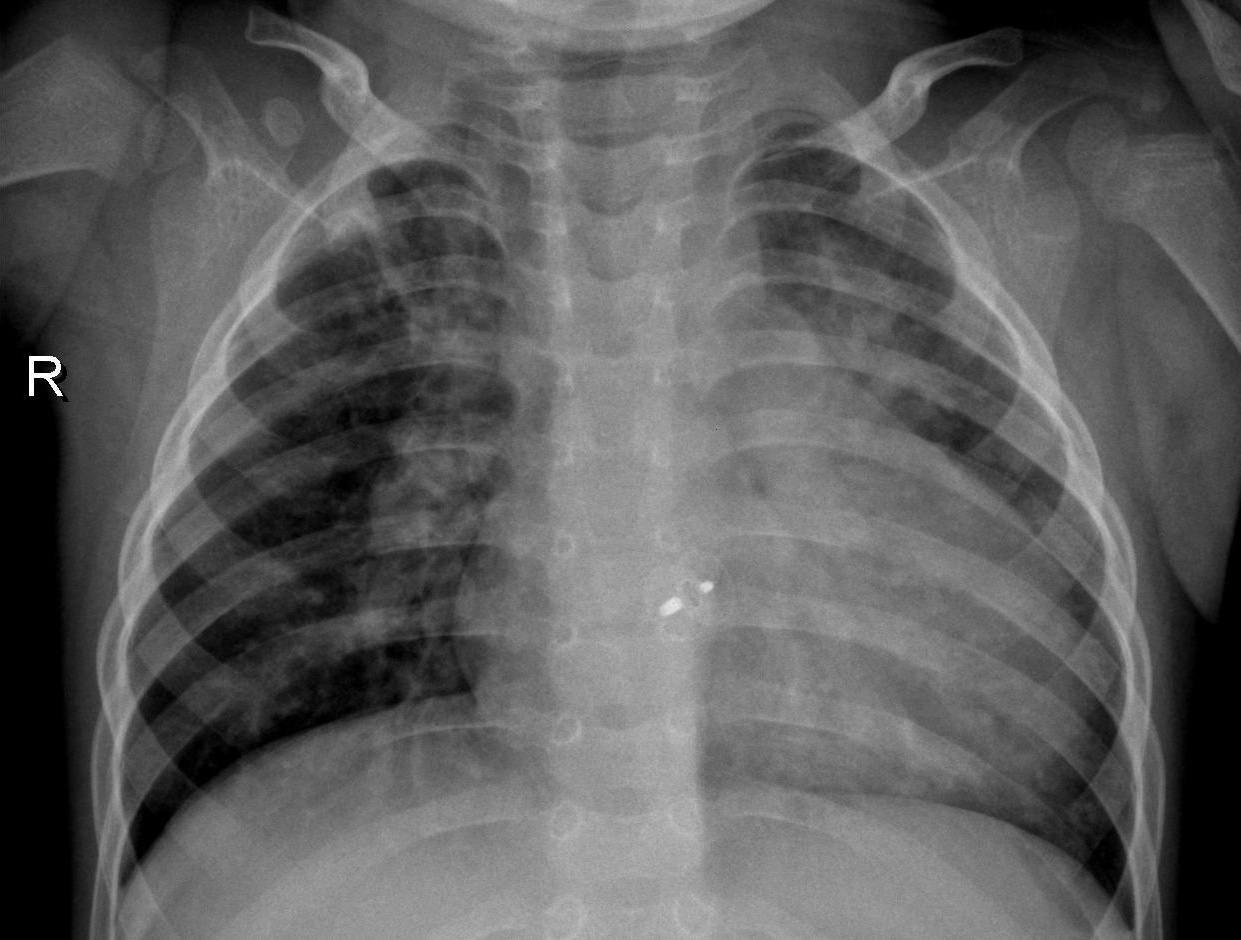
\includegraphics[width=\linewidth, height=30mm]{Images/PneumoniaOrig2.jpg}
    \vspace{0.5em}
    \end{minipage}
    &
  \begin{minipage}{.3\textwidth}
      \vspace{1em}
      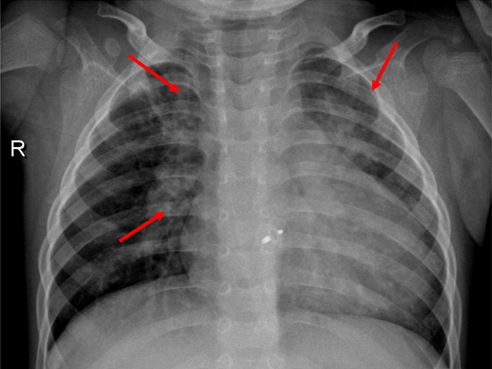
\includegraphics[width=\linewidth, height=30mm]{Images/PneuRadio2.png}
           \centering  Pneumonia
               \vspace{0.5em}
    \end{minipage}
    & 
    \begin{minipage}{.3\textwidth}
        \vspace{1em}
      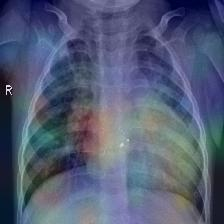
\includegraphics[width=\linewidth, height=30mm]{Images/PneuHeatmap2.jpg}
      \centering Pneumonia
          \vspace{0.5em}
    \end{minipage}
    \\ \hline
    \begin{minipage}{.3\textwidth}
    \vspace{1em}
      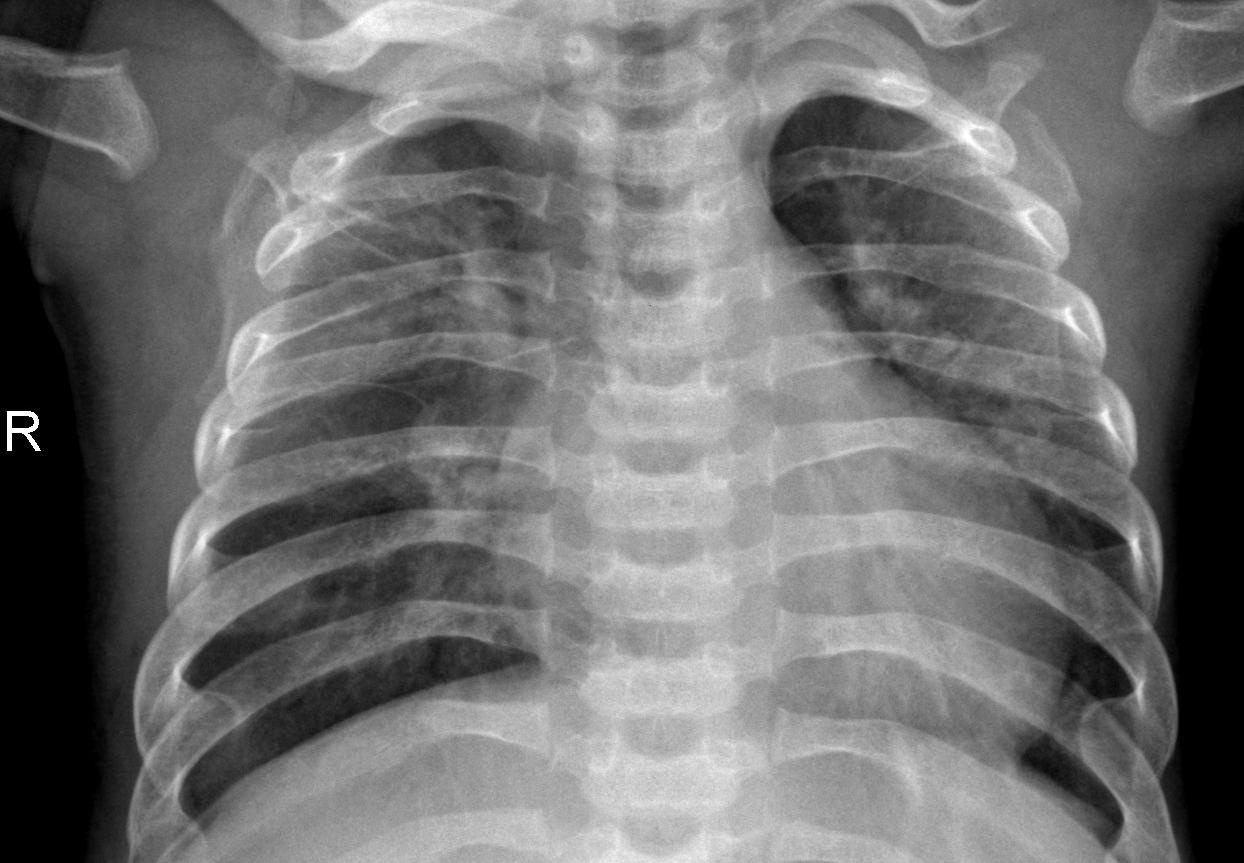
\includegraphics[width=\linewidth, height=30mm]{Images/PneuOrig3.jpg}
    \vspace{0.5em}
    \end{minipage}
    &
  \begin{minipage}{.3\textwidth}
      \vspace{1em}
      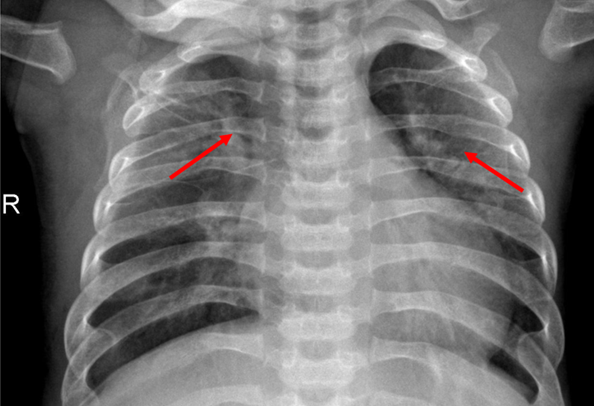
\includegraphics[width=\linewidth, height=30mm]{Images/PneuRadio3.png}
           \centering  Pneumonia
               \vspace{0.5em}
    \end{minipage}
    & 
    \begin{minipage}{.3\textwidth}
        \vspace{1em}
      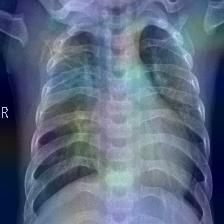
\includegraphics[width=\linewidth, height=30mm]{Images/PneuHeatmap3.jpg}
      \centering Pneumonia
          \vspace{0.5em}
    \end{minipage}
    \\ \hline
%       \begin{minipage}{.3\textwidth}
%     \vspace{1em}
%       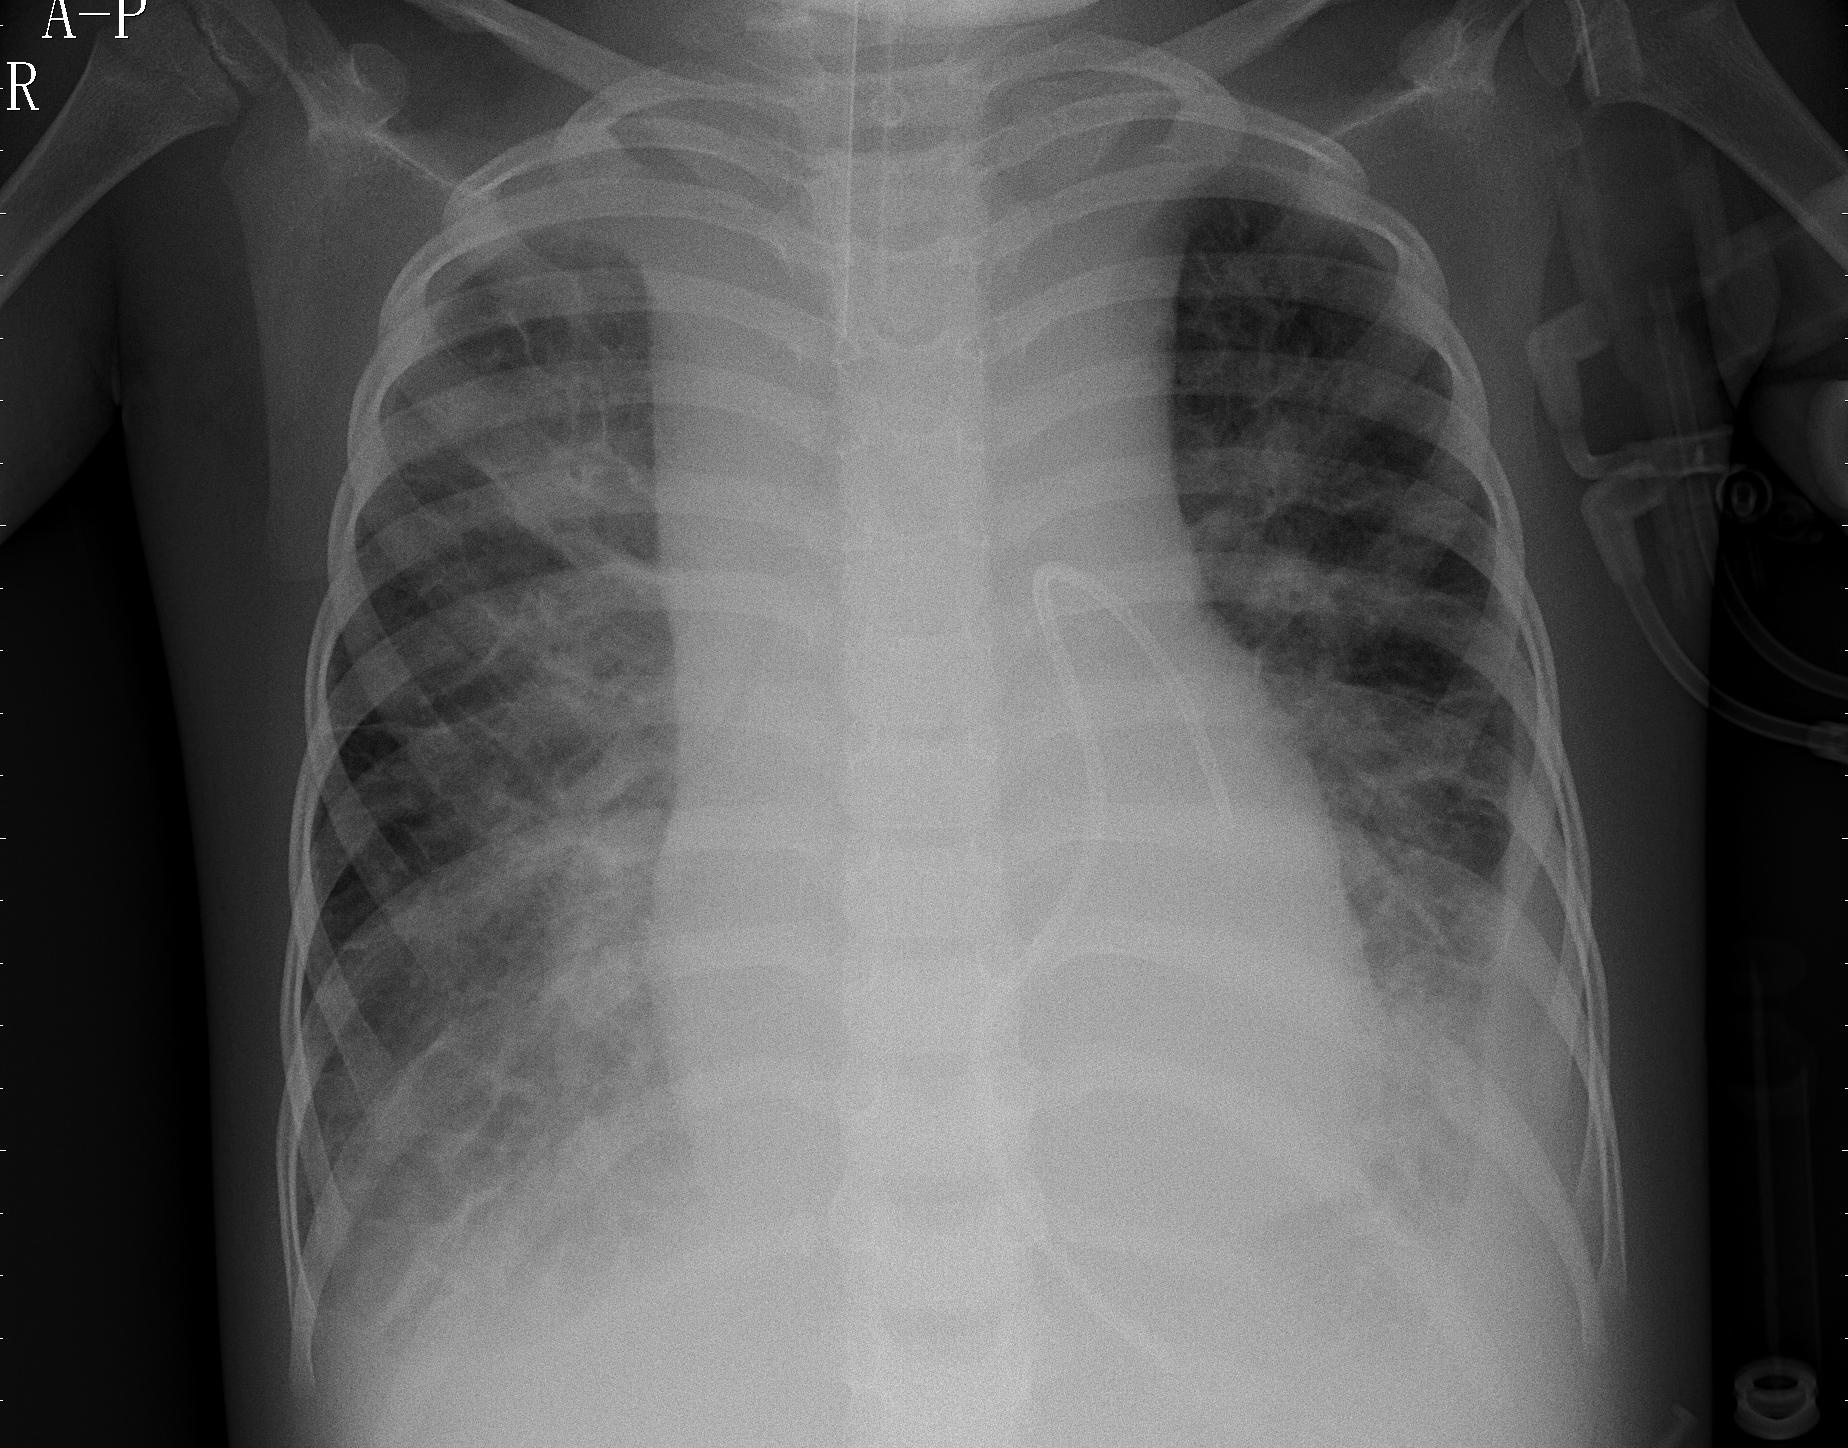
\includegraphics[width=\linewidth, height=30mm]{Images/PneuOrig4.jpg}
%     \vspace{0.5em}
%     \end{minipage}
%     &
%   \begin{minipage}{.3\textwidth}
%       \vspace{1em}
%       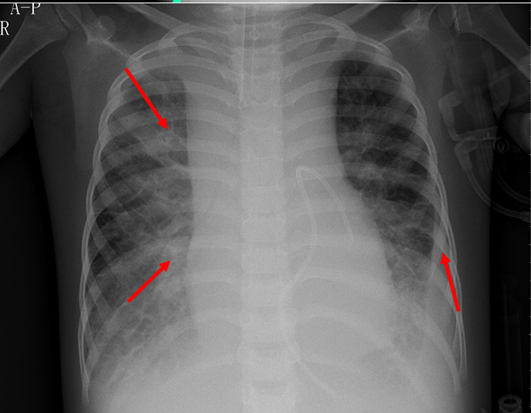
\includegraphics[width=\linewidth, height=30mm]{Images/PneuRadio4.png}
%           \centering  Pneumonia
%               \vspace{0.5em}
%     \end{minipage}
%     & 
%     \begin{minipage}{.3\textwidth}
%         \vspace{1em}
%       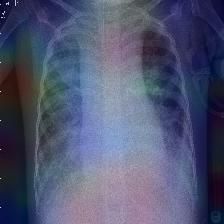
\includegraphics[width=\linewidth, height=30mm]{Images/PneuHeatmap4.jpg}
%       \centering Pneumonia
%           \vspace{0.5em}
%     \end{minipage}
    % \\ \hline
          \begin{minipage}{.3\textwidth}
    \vspace{1em}
      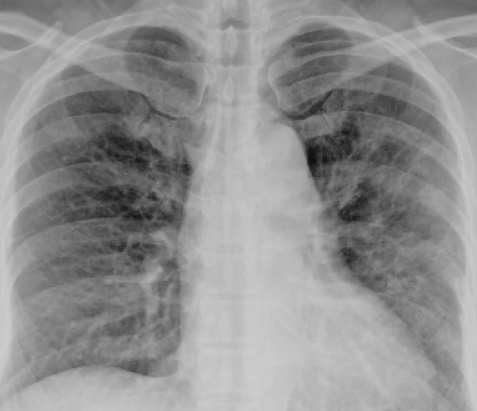
\includegraphics[width=\linewidth, height=30mm]{Images/covidOrig1.jpg}
    \vspace{0.5em}
    \end{minipage}
    &
  \begin{minipage}{.3\textwidth}
      \vspace{1em}
      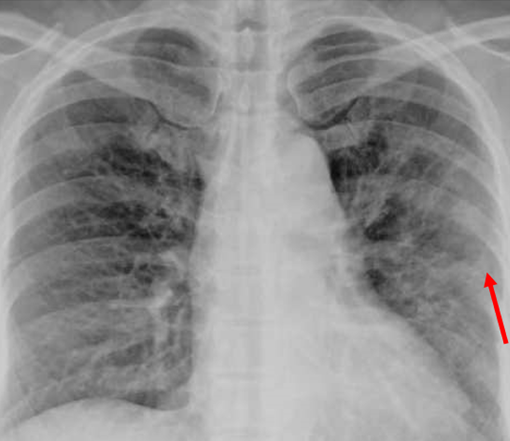
\includegraphics[width=\linewidth, height=30mm]{Images/covidRadio1.png}
           \centering  COVID-19
               \vspace{0.5em}
    \end{minipage}
    & 
    \begin{minipage}{.3\textwidth}
        \vspace{1em}
      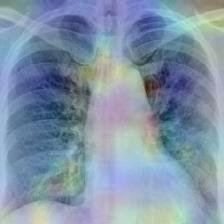
\includegraphics[width=\linewidth, height=30mm]{Images/covidHeatmap1.jpg}
      \centering COVID-19
          \vspace{0.5em}
    \end{minipage}
    \\ \hline
          \begin{minipage}{.3\textwidth}
    \vspace{1em}
      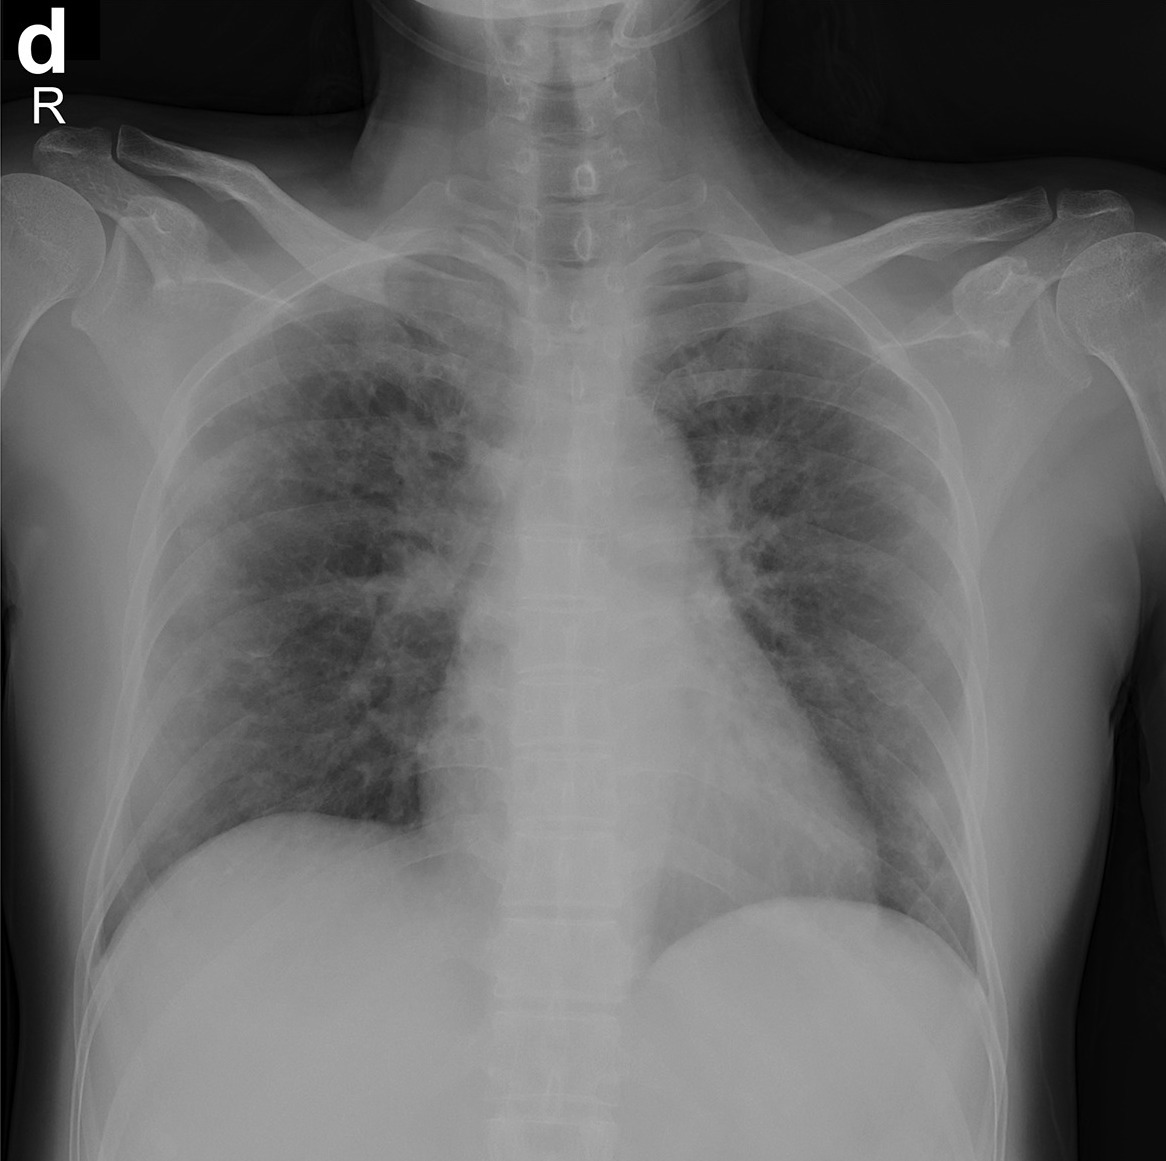
\includegraphics[width=\linewidth, height=30mm]{Images/covidOrig2.jpg}
    \vspace{0.5em}
    \end{minipage}
    &
  \begin{minipage}{.3\textwidth}
      \vspace{1em}
      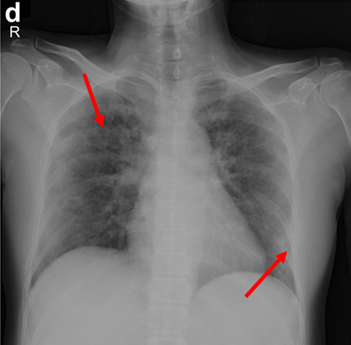
\includegraphics[width=\linewidth, height=30mm]{Images/covidRadio2.png}
           \centering  COVID-19
               \vspace{0.5em}
    \end{minipage}
    & 
    \begin{minipage}{.3\textwidth}
        \vspace{1em}
      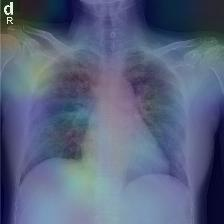
\includegraphics[width=\linewidth, height=30mm]{Images/covid19Heatmap2.jpg}
      \centering COVID-19
          \vspace{0.5em}
    \end{minipage}
    \\ \hline
  \caption{Comparison with Radiologist Finding}\label{tab:radioFinding}
\end{longtable}



\section{CT Scans}

In this section we conduct a comprehensive evaluation and comparison of the performance across each of our CT models.
    \vspace{-1em}
\subsection{Performance Evaluation}

The following sections evaluates the performance of each of our base models, UNet, Attention UNet, and UNet++. We have supplemented these sections with tables, plots indicating the trends in loss and accuracy, and confusion matrices respectively. 
    \vspace{-1em}

\subsubsection{Pre-trained Models}

The first model we have experimented with is UNet. We have achieved an average accuracy of 94.9\% after performing 10-fold cross validation on the balanced dataset. The average and best accuracy obtained on unseen data are 94.6\% and 95.7\% respectively. The classification report, confusion matrix, and trends in accuracy and loss have been displayed in Table \ref{tab:UNet CR}, Figure \ref{fig:UNet Confusion Matrix}, and Figure \ref{fig:unetModelTraining} respectively.

    % \vspace{1em}

\begin{table}[ht]
\begin{minipage}[b]{0.55\linewidth}
\centering
  \begin{longtable}{| p{.21\textwidth} |  p{.17\textwidth} |   p{.13\textwidth} | p{.11\textwidth} |} 
    \hline
& \textbf{Precision} & \textbf{Recall}    & \textbf{F1-Score}  \\
\hline
			COVID-19    &95.2\%   &94.7\%    &94.9\%
\\\hline
			Normal      &94.7\%   &95.2\%    &94.9\%
\\\hline 

    \end{longtable}
        \vspace{0.5em}
    \begin{longtable}{| p{.52\textwidth} |  p{.13\textwidth}|} 
    \hline
    		\textbf{Accuracy}    &94.9\%
\\\hline
        \end{longtable}

    \vspace{1em}
     \captionsetup{width=.8\linewidth}

 \caption{UNet Model Classification Report}  \label{tab:UNet CR}
\end{minipage}
\begin{minipage}[b]{0.45\linewidth}
\centering
 \captionsetup{width=.8\linewidth}
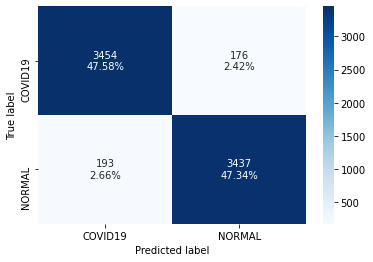
\includegraphics[width=1\linewidth]{Images/UNetCM.png}
\captionof{figure}{UNet Model Confusion Matrix}
\label{fig:UNet Confusion Matrix}
\end{minipage}
\end{table}

\vspace{-\parskip}
\begin{figure}[H]
        \begin{subfigure}[b]{0.5\textwidth}
                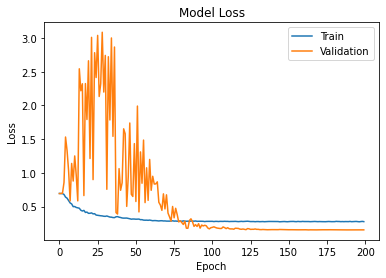
\includegraphics[width=\linewidth]{Images/UNetAcc.png}
        \end{subfigure}%
        \begin{subfigure}[b]{0.5\textwidth}
                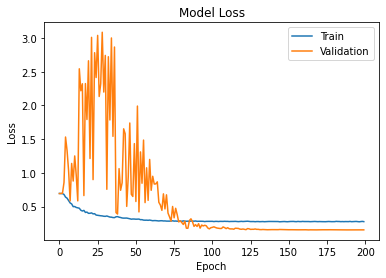
\includegraphics[width=\linewidth]{Images/UNetLoss.png}
        \end{subfigure}%
        %\\\centering
            %\decoRule
        \caption{UNet Model Training Performance Trends}\label{fig:unetModelTraining}
\end{figure}

Next, we trained our Attention UNet model. We achieved an average accuracy of 98.1\% after 10-fold cross validation on the balanced dataset. The average and best accuracy obtained on the unseen data are 98.3\% and 99.2\%. We have displayed the classification report, confusion matrix, and trends in accuracy and loss in Table \ref{tab:Att UNet CR}, Figure \ref{fig:Att UNet Confusion Matrix}, and Figure \ref{fig:attunetModelTraining} respectively.

    \vspace{1em}

\begin{table}[ht]
\begin{minipage}[b]{0.55\linewidth}
\centering
  \begin{longtable}{| p{.21\textwidth} |  p{.17\textwidth} |   p{.13\textwidth} | p{.11\textwidth} |} 
    \hline
& \textbf{Precision} & \textbf{Recall}    & \textbf{F1-Score}  \\
\hline
			COVID-19    &98.3\%   &97.9\%    &98.1\%
\\\hline
			Normal      &97.9\%   &98.3\%    &98.1\%
\\\hline 

    \end{longtable}
        \vspace{0.5em}
    \begin{longtable}{| p{.52\textwidth} |  p{.13\textwidth}|} 
    \hline
    		\textbf{Accuracy}    &98.1\%
\\\hline
        \end{longtable}

    \vspace{1em}
     \captionsetup{width=.8\linewidth}

 \caption{Attention UNet Model Classification Report}  \label{tab:Att UNet CR}
\end{minipage}
\begin{minipage}[b]{0.45\linewidth}
\centering
 \captionsetup{width=.8\linewidth}

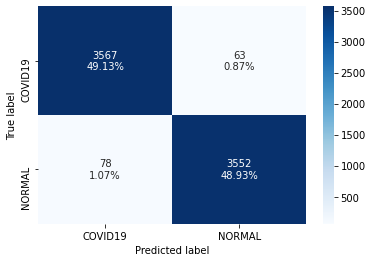
\includegraphics[width=1\linewidth]{Images/AttUNetCM.png}
\captionof{figure}{Attention UNet Model Confusion Matrix}
\label{fig:Att UNet Confusion Matrix}
\end{minipage}
\end{table}
\vspace{-\parskip}

\begin{figure}[H]
        \begin{subfigure}[b]{0.5\textwidth}
                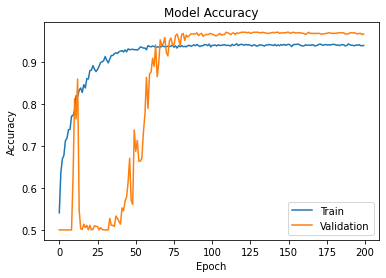
\includegraphics[width=\linewidth]{Images/AttUNetAccuracy.png}
        \end{subfigure}%
        \begin{subfigure}[b]{0.5\textwidth}
                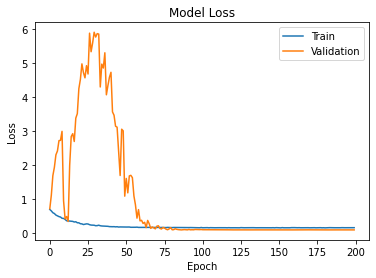
\includegraphics[width=\linewidth]{Images/AttUNetLoss.png}
        \end{subfigure}%
        %\\\centering
            %\decoRule
        \caption{Attention UNet Model Training Performance Trends}\label{fig:attunetModelTraining}
\end{figure}

The last model we have evaluated is UNet++. We have achieved an average accuracy of 90.2\% after 10-fold cross validation on the balanced dataset. The average and best accuracy obtained on the unseen data are 88.0\% and 91.2\% respectively. We have displayed the classification report, confusion matrix, and trends in loss and accuracy in Table \ref{tab:UNet++ CR}, Figure \ref{fig:UNet++ Confusion Matrix}, and Figure \ref{fig:unet++ModelTraining} respectively.


    % \vspace{1em}

\begin{table}[ht]
\begin{minipage}[b]{0.55\linewidth}
\centering
  \begin{longtable}{| p{.21\textwidth} |  p{.17\textwidth} |   p{.13\textwidth} | p{.11\textwidth} |} 
    \hline
& \textbf{Precision} & \textbf{Recall}    & \textbf{F1-Score}  \\
\hline
			COVID-19    &92.9\%   &88.1\%    &90.5\%
\\\hline
			Normal      &88.1\%   &92.9\%    &90.5\%
\\\hline 

    \end{longtable}
        \vspace{0.5em}
    \begin{longtable}{| p{.52\textwidth} |  p{.13\textwidth}|} 
    \hline
    		\textbf{Accuracy}    &90.2\%
\\\hline
        \end{longtable}

    \vspace{1em}
     \captionsetup{width=.7\linewidth}

 \caption{UNet++ Model Classification Report}  \label{tab:UNet++ CR}
\end{minipage}
\begin{minipage}[b]{0.45\linewidth}
\centering
 \captionsetup{width=.8\linewidth}

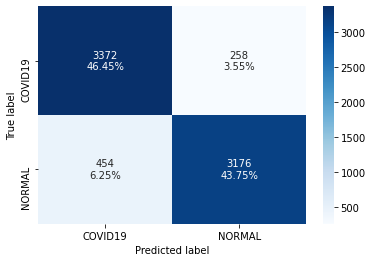
\includegraphics[width=1\linewidth]{Images/UNet++CM.png}
\captionof{figure}{UNet++ Model Confusion Matrix}
\label{fig:UNet++ Confusion Matrix}
\end{minipage}
\end{table}
\vspace{-\parskip}
\begin{figure}[H]
        \begin{subfigure}[b]{0.5\textwidth}
                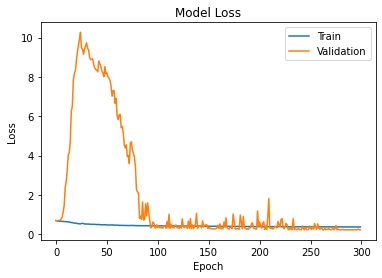
\includegraphics[width=\linewidth]{Images/UNet++Accuracy.png}
        \end{subfigure}%
        \begin{subfigure}[b]{0.5\textwidth}
                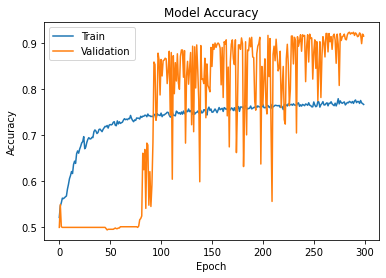
\includegraphics[width=\linewidth]{Images/UNet++Loss.png}
        \end{subfigure}%
        %\\\centering
            %\decoRule
        \caption{UNet++ Model Training Performance Trends}\label{fig:unet++ModelTraining}
\end{figure}

\vspace{-3em}
\subsubsection{Ensemble Model}

We have ensembled each of our base CT models to further improve classification performance. We have achieved an average accuracy of 98.7\% after cross validation of the balanced dataset. The average and best accuracy obtained on unseen data are 97.9\% and 97.8\%. Table \ref{tab:CT Ensemble CR}, Figure \ref{fig:CT Ensemble Confusion Matrix}, and Figure \ref{fig:ctensembleModelTraining} displays the classification report, confusion matrix, and trends in loss and accuracy respectively.



    % \vspace{1em}

\begin{table}[ht]
\begin{minipage}[b]{0.55\linewidth}
\centering
  \begin{longtable}{| p{.21\textwidth} |  p{.17\textwidth} |   p{.13\textwidth} | p{.11\textwidth} |} 
    \hline
& \textbf{Precision} & \textbf{Recall}    & \textbf{F1-Score}  \\
\hline
			COVID-19    &98.8\%   &98.5\%    &98.7\%
\\\hline
			Normal      &98.5\%   &98.8\%    &98.7\%
\\\hline 

    \end{longtable}
        \vspace{0.5em}
    \begin{longtable}{| p{.52\textwidth} |  p{.13\textwidth}|} 
    \hline
    		\textbf{Accuracy}    &98.7\%
\\\hline
        \end{longtable}
 \captionsetup{width=.8\linewidth}

    \vspace{1em}
 \caption{CT Ensemble Model Classification Report}  \label{tab:CT Ensemble CR}
\end{minipage}
\begin{minipage}[b]{0.45\linewidth}
\centering
 \captionsetup{width=.8\linewidth}

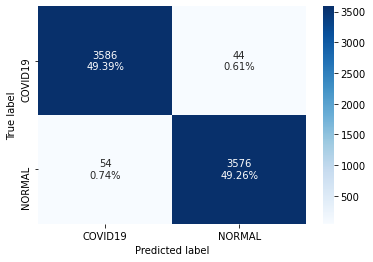
\includegraphics[width=1\linewidth]{Images/CTEnsembleCM.png}
\captionof{figure}{CT Ensemble Model Confusion Matrix}
\label{fig:CT Ensemble Confusion Matrix}
\end{minipage}
\end{table}


\begin{figure}[H]
        \begin{subfigure}[b]{0.5\textwidth}
                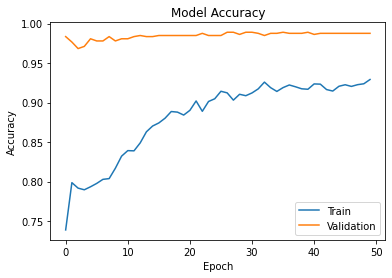
\includegraphics[width=\linewidth]{Images/CTEnsembleAccuracy.png}
        \end{subfigure}%
        \begin{subfigure}[b]{0.5\textwidth}
                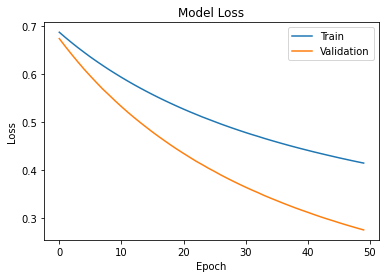
\includegraphics[width=\linewidth]{Images/CTEnsembleLoss.png}
        \end{subfigure}%
        %\\\centering
            %\decoRule
        \caption{CT Ensemble Model Training Performance Trends}\label{fig:ctensembleModelTraining}
\end{figure}


\subsection{Performance Comparison}

In the following sections, we compare our models amongst each other and determine the best model. We also compare the best model with the RT-PCR test and CNN, followed by similar studies from literature. Finally, we compare the heatmaps obtained with findings observed by a professional Radiologist.

\subsubsection{Trained Models}

We compare each of our base CT models along with the ensemble model across various parameters such as Accuracy, Precision, Recall, F1-Score, Specificity, and Sensitivity respectively. These metric scores are tabulated in Table \ref{tab:mpcCT}.

\vspace{1em}
 \begin{longtable}{| p{.23\textwidth} |  p{.1\textwidth} |   p{.1\textwidth} | p{.06\textwidth} | p{.095\textwidth} | p{.11\textwidth} | p{.11\textwidth} |} 
    \hline
& \textbf{Accuracy} & \textbf{Precision} & \textbf{Recall} & \textbf{F1-Score} & \textbf{Specificity} & \textbf{Sensitivity} \\
\hline
			UNet    &94.9\%   &94.9\%    &94.9\%    &94.9\%   &94.9\%   &94.9\% 
\\\hline
			Attention UNet    &98.1\%   &98.1\%    &98.1\%    &98.1\%   &98.1\%   &98.1\% 
\\\hline
			UNet++    &90.2\%   &90.5\%    &90.5\%    &90.5\%   &90.3\%   &90.5\% 
\\\hline
	        \textbf{Ensemble Model}    &\textbf{98.7\%}   &\textbf{98.7\%}    &\textbf{98.7\%}    &\textbf{98.7\%}   &\textbf{98.7\%}   &\textbf{98.7\%} 
\\\hline
 \caption{CT Models Performance Comparison}  \label{tab:mpcCT}

    \end{longtable}
\vspace{-1em}
We observe that out of the base models, Attention UNet outperforms the rest. As expected, a slight performance increase is also observed from the Ensemble model.

\subsubsection{RT-PCR and CNN}

We compare the results obtained by our Ensemble model with traditional RT-PCR test and a basic CNN model, only for \textbf{COVID-19 class}. Once again, we use the study conducted by the Infectious Diseases Society of America (IDSA) \cite{IDS2020} for comparison purposes. Table \ref{tab:compCT} compares the results.

 \begin{longtable}{| p{.15\textwidth} | p{.11\textwidth} |  p{.11\textwidth} |   p{.11\textwidth} |} 
    \hline
& \textbf{Accuracy} & \textbf{Sensitivity} & \textbf{Specificity} \\
\hline

			RT-PCR      &-   &84.2\%    &98.9\%  
\\\hline
			CNN    &82.3\%   &80.2\%    &84.6\% 
\\\hline
			\textbf{Our Approach}   &\textbf{98.7\%}   &\textbf{98.5\%}    &\textbf{98.8\%} 
\\\hline
 \caption{Comparison with RT-PCR and CNN for X-ray scans}  \label{tab:compCT}
    \end{longtable}
\vspace{-1em}

We observe that our Ensemble model outperforms CNN across all metrics. Our approach also perform better than traditional RT-PCR test in terms of Sensitivity and has comparable Specificity.  

\subsubsection{Related Work}

We compare the performance of our Ensemble model to related work discussed in Section \ref{LR} across various metrics. The results are summarized in Table \ref{tab:relWorkCT}.


\vspace{1em}
 \begin{longtable}{| p{.23\textwidth} |  p{.1\textwidth} |   p{.1\textwidth} | p{.06\textwidth} | p{.095\textwidth} | p{.11\textwidth} | p{.11\textwidth} |} 
    \hline
& \textbf{Accuracy} & \textbf{Precision} & \textbf{Recall} & \textbf{F1-Score} & \textbf{Specificity} & \textbf{Sensitivity} \\
\hline
Wang et al. \cite{WBX+2020} &79.3\%    &55.0\%     &83.0\%   &66.2\%    &67.0\%     &83.0\%
\\\hline
Jin et al. \cite{JCW+2020} &80.4\%    &95.0\%     &73.5\%   &82.9\%    &92.9\%     &73.5\%
\\\hline
Song et al. \cite{SZL+2020} &86.0\%    &81.0\%     &93.0\%   &86.6\%    &76.7\%     &93.0\%
\\\hline
Zheng et al. \cite{CXZ+2020}   &90.1\%    &84.0\%     &90.7\%   &87.2\%    &91.1\%     &90.7\%
\\\hline
Chen et al. \cite{CJL+2020}   &91.6\%    &84.6\%     &100\%   &91.6\%    &93.6\%     &100\%
\\\hline
Li et al. \cite{LLL+2020}   &94.0\%    &89.7\%     &89.7\%   &89.7\%    &95.7\%     &89.7\%
\\\hline
% Jin et al. \cite{JSB+2020}  &\%    &\%     &\%   &\%    &92.2\%     &97.4\%
% \\\hline
\textbf{Ensemble Model}    &\textbf{98.7\%}   &\textbf{98.7\%}    &\textbf{98.7\%}    &\textbf{98.7\%}   &\textbf{98.7\%}   &\textbf{98.7\%} 
\\\hline
 \caption{Comparison with Related Work}  \label{tab:relWorkCT}

    \end{longtable}
\vspace{-1em}

Our Ensemble model performs significantly better when compared other approaches across all metrics. Once again, the data pre-processing and processing workflow such as splitting the lung parenchyma, augmentation, transfer learning, and ensemble learning respectively, seems to play a major factor to the models optimal performance.


\subsubsection{Radiologist Findings}

We once again compare the generated heatmaps with that of the findings observed by a professional Radiologist. From Table \ref{tab:radioFindingCT}, we can observe that the heatmaps generated are in direct conformance with the senior Radiologist's finding \footnote{The authors thank Dr. G.R. Mahadevan (MD, IDCCM,D.Diab, Specialist in COVID-19) from Maya Nursing Home,Tamil Nadu for annotating the X-ray and CT images.}. The heatmaps identify atleast one or more of the critical regions highlighted by the Radiologist. We also observe that all areas highlighted by the Radiologist are shades of red, purple, or green and not blue. 

Furthermore, similar to our observations from Section \ref{rfxray}, we have verfied that our heatmaps correlate to the studies conducted by Harmon et al., Li et al., and Chung et al., therefore ensuring the reliability of our results. We observe that consolidations, GGO's, and lesions are major contributing factors to COVID-19 detection.

\begin{longtable} { | c | c | c | }
    \hline
    \textbf{Original} & \textbf{Radiologist Finding} & \textbf{Heatmap} \\ \hline
    \begin{minipage}{.3\textwidth}
    \vspace{1em}
      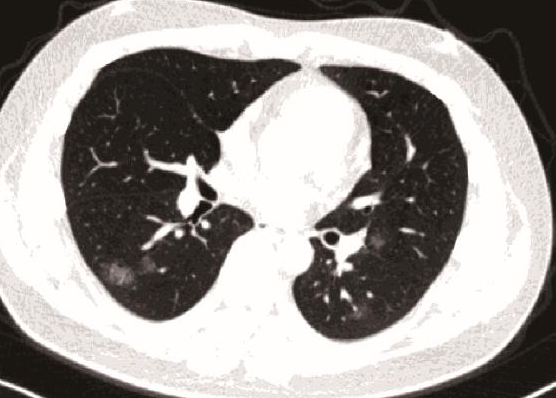
\includegraphics[width=\linewidth, height=30mm]{Images/ctOrig1.png}
    \vspace{0.5em}
    \end{minipage}
    &
  \begin{minipage}{.3\textwidth}
      \vspace{1em}
      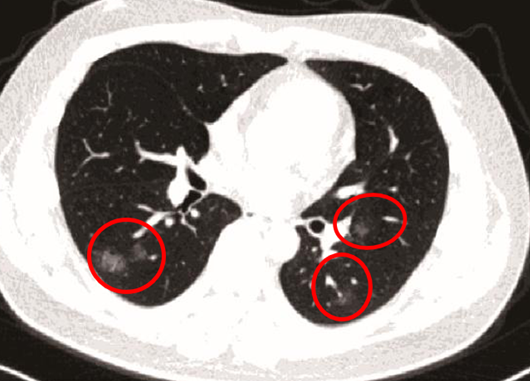
\includegraphics[width=\linewidth, height=30mm]{Images/ctRadio1.png}
           \centering  COVID-19
               \vspace{0.5em}
    \end{minipage}
    & 
    \begin{minipage}{.3\textwidth}
        \vspace{1em}
      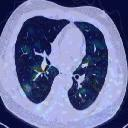
\includegraphics[width=\linewidth, height=30mm]{Images/ctHeatmap1.jpg}
      \centering COVID-19
          \vspace{0.5em}
    \end{minipage}
    \\ \hline
    \begin{minipage}{.3\textwidth}
    \vspace{1em}
      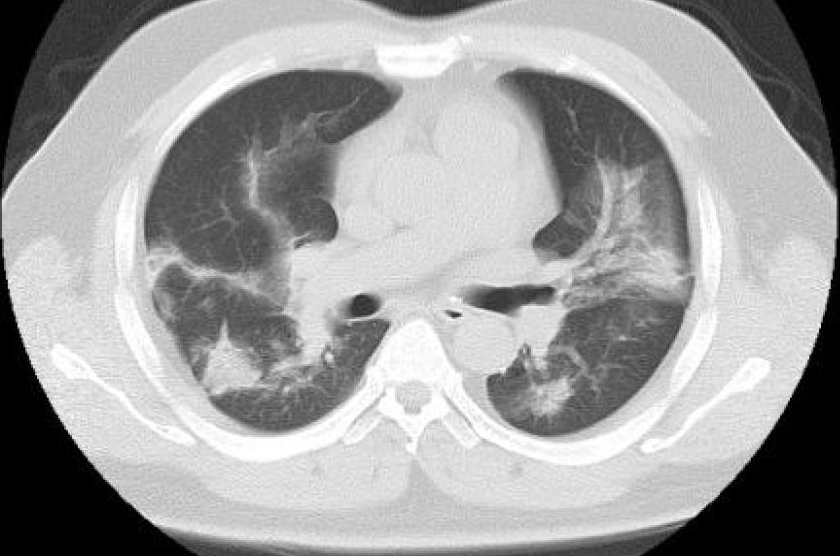
\includegraphics[width=\linewidth, height=30mm]{Images/ctOrig2.png}
    \vspace{0.5em}
    \end{minipage}
    &
  \begin{minipage}{.3\textwidth}
      \vspace{1em}
      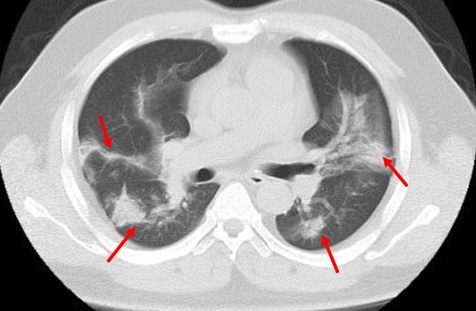
\includegraphics[width=\linewidth, height=30mm]{Images/ctRadio2.png}
           \centering  COVID-19
               \vspace{0.5em}
    \end{minipage}
    & 
    \begin{minipage}{.3\textwidth}
        \vspace{1em}
      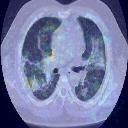
\includegraphics[width=\linewidth, height=30mm]{Images/ctHeatmap2.jpg}
      \centering COVID-19
          \vspace{0.5em}
    \end{minipage}
     \\ \hline
    \begin{minipage}{.3\textwidth}
    \vspace{1em}
      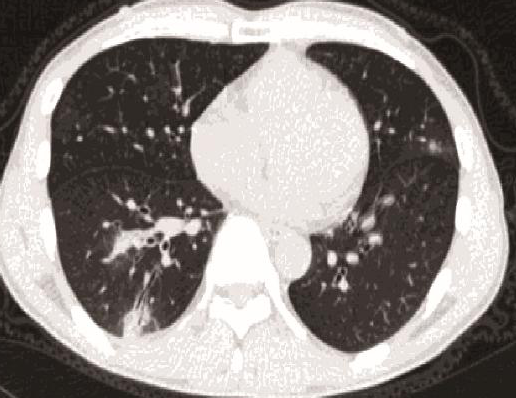
\includegraphics[width=\linewidth, height=30mm]{Images/ctOrig3.png}
    \vspace{0.5em}
    \end{minipage}
    &
  \begin{minipage}{.3\textwidth}
      \vspace{1em}
      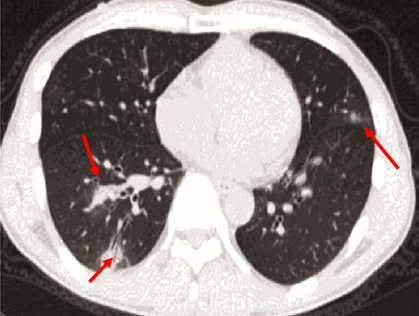
\includegraphics[width=\linewidth, height=30mm]{Images/ctRadio3.png}
           \centering  COVID-19
               \vspace{0.5em}
    \end{minipage}
    & 
    \begin{minipage}{.3\textwidth}
        \vspace{1em}
      \includegraphics[width=\linewidth, height=30mm]{Images/ctHeatmap3.jpg}
      \centering COVID-19
          \vspace{0.5em}
    \end{minipage}
      \\ \hline
  \caption{Comparison with Radiologist Finding}\label{tab:radioFindingCT}

\end{longtable}

\section{Web Interface}
In this section, we highlight the results obtained by the Usability Study we have conducted. It is of utmost importance to understand and measure the usability of the COVID-19 and Pneumonia Diagnosis Platform. The feedback received would be really beneficial for future iterations of this application in terms of design improvements and feature additions.

\subsection{Hypothesis} \label{hypo}

\textit{Through this experiment, Alister George Luiz (the investigator) is attempting to prove that the
COVID-19 and Pneumonia Diagnosis Platform is usable in the sense that it is user-friendly, consistent, familiar, responsive, and intuitive.}

\subsection{Target Audience}

Any user, with or without technical experience, in any age group was eligible for this study. A consent form was provided virtually to comply with the compulsory policy of no face-to-face interactions due to the outbreak of the pandemic. All the terms and conditions were presented before the participant undertook the survey and was given freedom to accept or decline participation. The consent form was taken from the resources provided by the F20PA course page.

\subsection{Experiment Design}
The main motive behind designing a Usability Study was due to the fact that the COVID-19 and Pneumonia Diagnosis Platform is a user-facing product. The purpose of this user study was to \textbf{quantitatively} and \textbf{qualitatively} understand the perspective of the user towards our final product. Our experiment is composed of three activities. The investigator ensured that the participants viewed the video demonstration of the Diagnosis Portal and also provided Screenshots covering all aspects of the website. We have utilized Microsoft Forms  \footnote{The Microsoft Forms Link containing the Survey can be found here: \url{https://forms.office.com/r/vFuJ0VCXe5}} to conduct this study.

\subsection{Activity 1: Tasks}

In the first activity, we have asked the participants several questions after they have viewed the video demonstration. The goal of this activity was to verify that the basic system functionality is easily understandable and that they could perform these tasks without intervention from the investigator or any similar secondary help. 

The outcome of each question was either a yes or no to evaluate the participants understandability. Besides this, the investigator also welcomed feedback on the existing systems, which may be considered in future versions of this Web Portal. It is worth to note that participants were given a brief explanation of the project in the beginning of the study, and any questions were welcome via email or other messaging sources. 

We have asked this question to participants before the activity - \textbf{How frequently do you use a Computer?}

All users provided 'Daily' as their response. The main purpose of this question was to understand the influence of familiarity with computers in their respective ease of understanding of the system. We found that 
participants with daily usage of computers are usually more technically adept and can easily comprehend the system workflow. Table \ref{act:1} displays the questions and results obtained for Activity 1. 

\begin{longtable}{| p{.055\textwidth} | p{.75\textwidth} | p{.04\textwidth} | p{.03\textwidth} |} 
    \hline
    		\textbf{Q.No}    &\textbf{Question} & \textbf{Yes}     & \textbf{No}
\\\hline
            1   &Would you be able to utilize the functionality of this website independently?  &15  &0
\\\hline
            2   &Were you able to comprehend the Disclaimer message easily?  &15  &0
\\\hline
            3   &Were you able to identify where to upload the scan easily?  &15  &0
\\\hline
            4   &Were you able to understand that the slideshow showcased previous diagnosis results obtained from the portal for both COVID-19 and Pneumonia?  &13  &2
\\\hline
            5   &Were you able to identify the use of the toggle button between X-ray and CT scan?  &15  &0
\\\hline

\caption{Activity 1 Results} \label{act:1}
        \end{longtable}

The results obtained indicates that most of the participants easily understood the basic functionality and workflow of this Diagnosis Portal. Three participants could not recognize that the Gallery section showcased previous diagnosis results obtained from the portal. We believe adding a more explicit description would help in better understanding of the Gallery section.

Besides these questions, the participant was also asked to provide feedback if they felt so regarding the interface or any general suggestions. Table \ref{feedback} highlights some of the top suggestions provided, which would be definitely considered in future versions of this Diagnosis Portal.


\begin{longtable}{| p{.055\textwidth} | p{.83\textwidth} |} 
    \hline
    		\textbf{S.No}    &\textbf{Suggestions for Improvement} 
\\\hline
            1   &Improvements to UI, Multi-page Site as in separate page for COVID-19 and Pneumonia
\\\hline
            2   &Just keep adjusting the layout of the website so rather than scrolling all site content are seen together. Also since it's a diagnosis web portal, for future works integrating different medical issues related to COVID-19 can be trained in the AI, for more efficient outcomes
\\\hline
            3   &If the result of the diagnosis indicates COVID - 19, guidelines and measures (according to region) being presented along with it would be helpful.
\\\hline
          4   &The options for switching between X-ray and CT could be renamed as "Click here to view X-ray" and "Click here to view CT Scan"
\\\hline

\caption{Feedback on the Diagnosis Portal} \label{feedback}
        \end{longtable}

It is indeed possible to extract relevant functionality improvements from the general feedback. Revision in User Interface, adding more information related to COVID-19, providing guidelines and measures pertaining to the region and so on are high in our priority list. We thank the participants for providing such valuable feedback.

\subsection{Activity 2: System Usability Scale (SUS) Survey}

Next, we have utilized the System Usability Scale which is a renowned and widely used tool to measure the usability of the system \cite{SUS2021, JBR1986}. We successfully completed the usability testing with fifteen participants. 

The System Usability Scale (SUS) comprised of ten questions. Each participant had to provide a rating between 1 to 5 which indeed correlated to \textbf{Strongly Disagree} and \textbf{Strongly Agree}. One interesting aspect of using the SUS was that we could easily average out the results from each participant and obtain the general consensus. The standard SUS formula was used to compute the final scores \cite{THO2015} for each participant. The questions are displayed in Table \ref{susQ} and the results obtained from each participant along with the scores is provided in Table \ref{susScores}.

\begin{longtable}{| p{.055\textwidth} | p{.83\textwidth} |} 
    \hline
    		\textbf{Q.No}    &\textbf{Question} 
\\\hline
            1   &I think that I would like to use this system frequently. Given that feedback on the results obtained by the portal must be validated by a medical professional. 
\\\hline
2   &I found this system unnecessarily complex. 
\\\hline
3   &I thought this system was easy to use. 
\\\hline
4   &I think that I would need assistance to be able to use the system. 
\\\hline
5   &I found the various functions in this system were well integrated. 
\\\hline
6   &I thought there was too much inconsistency in this system. 
\\\hline
7   &I would imagine that most people would learn to use this system very quickly.
\\\hline
8   &I found this system very cumbersome/awkward to use.
\\\hline
9   &I feel very confident using this system.
\\\hline
10  &I needed to learn a lot of things before I could get going with this system.
\\\hline

\caption{System Usability Scale (SUS) Questions} \label{susQ}
        \end{longtable}
\vspace{-1em}
\begin{longtable}{| p{.12\textwidth} | p{.03\textwidth} | p{.03\textwidth} | p{.03\textwidth} | p{.03\textwidth} | p{.03\textwidth} | p{.03\textwidth} | p{.03\textwidth} | p{.03\textwidth} | p{.03\textwidth} | p{.04\textwidth} | p{.06\textwidth} |} 
    \hline
    		\textbf{Participant}    &\textbf{Q1}    &\textbf{Q2}    &\textbf{Q3}    &\textbf{Q4}    &\textbf{Q5}    &\textbf{Q6}   &\textbf{Q7}    &\textbf{Q8}    &\textbf{Q9}    &\textbf{Q10}   &\textbf{Score} 
\\\hline
P1   &4   &1   &4   &1   &5   &1   &5   &1   &4   &1   &92.5 \\\hline
P2   &5   &1   &5   &2   &4   &1   &4   &1   &5   &1   &92.5 \\\hline
P3   &5   &1   &5   &1   &5   &1   &5   &1   &5   &1   &100 \\\hline
P4   &5   &1   &5   &1   &5   &1   &4   &2   &5   &1   &95 \\\hline
P5   &5   &1   &5   &1   &3   &1   &5   &1   &5   &1   &95 \\\hline
P6   &5   &2   &5   &1   &5   &1   &5   &2   &5   &1   &95 \\\hline
P7   &3   &1   &4   &1   &3   &1   &3   &1   &3   &1   &77.5 \\\hline
P8   &5   &1   &5   &1   &5   &1   &5   &1   &5   &1   &100 \\\hline
P9   &4   &2   &4   &1   &3   &1   &4   &1   &4   &1   &95 \\\hline
P10  &5   &1   &5   &1   &4   &2   &5   &1   &5   &1   &95 \\\hline
P11  &5   &1   &5   &2   &5   &1   &4   &1   &4   &1   &92.5 \\\hline
P12  &5   &1   &5   &1   &5   &2   &5   &1   &5   &1   &97.5 \\\hline
P13  &2   &1   &4   &2   &3   &1   &4   &1   &4   &1   &77.5 \\\hline
P14  &4   &2   &5   &1   &4   &2   &4   &1   &3   &2   &80 \\\hline
P15  &3   &2   &4   &2   &4   &2   &4   &2   &3   &2   &70 \\\hline
\caption{System Usability Scale (SUS) Scores} \label{susScores}
\end{longtable}


The average SUS score is \textbf{90.3}. As per Jeff Sauro, a SUS score above 68 is \textbf{Above Average}. A score above 80.3 is \textbf{Excellent}. As per our this criteria, we are pleased to know that our Diagnosis Portal falls into the former category. Figure \ref{fig:susScore} displays our SUS scores and the average score. We also believe that the Mode statistical quantity is in fact really useful in understanding the participants general mindset. Therefore, we have highlighted the Mode, Maximum and Minimum per question in Table \ref{susStats}. 

\begin{figure}[H]
    \centering
    \includegraphics[height=7cm]{Images/SUSScore.png}
    %\decoRule
    \caption{Comparison of SUS Scores}
    \label{fig:susScore}
    \end{figure}
\begin{longtable}{| p{.11\textwidth} | p{.03\textwidth} | p{.03\textwidth} | p{.03\textwidth} | p{.03\textwidth} | p{.03\textwidth} | p{.03\textwidth} | p{.03\textwidth} | p{.03\textwidth} | p{.03\textwidth} | p{.04\textwidth} |} 
    \hline
    		\textbf{Statistic}    &\textbf{Q1}    &\textbf{Q2}    &\textbf{Q3}    &\textbf{Q4}    &\textbf{Q5}    &\textbf{Q6}   &\textbf{Q7}    &\textbf{Q8}    &\textbf{Q9}    &\textbf{Q10}   
\\\hline
Mode        &5   &1   &5   &1   &5   &1   &5   &1   &5   & 1 
\\\hline
Maximum     &5   &2   &5   &2   &5   &2   &5   &2   &5   &2  
\\\hline
Minimum     &2   &1   &4   &1   &3   &1   &3   &1   &3   &1  
\\\hline
\caption{System Usability Scale (SUS) Statistical Analysis} \label{susStats}
\end{longtable}

\subsection{Activity 3: Metrics Test}

The last activity involves explicitly testing the certain metrics stated in Section \ref{hypo} and Table \ref{tab:Evaluation Strategy}. We have asked the participants to fill in a Likert Scale which each metric having scores ranging from Very Poor to Excellent. Table \ref{metricTest} summarizes the results. 

\begin{longtable}{| p{.19\textwidth} | p{.11\textwidth} | p{.05\textwidth} | p{.04\textwidth} | p{.06\textwidth} | p{.10\textwidth} |} 
    \hline
    		\textbf{Metric}    &\textbf{Very Poor}    &\textbf{Poor}    &\textbf{Fair}    &\textbf{Good}    &\textbf{Excellent}
\\\hline
User-Friendliness  &0   &0   &1   &7  &7   
\\\hline
Consistency  &0   &0   &1   &8   &6  
\\\hline
Familiarity  &0   &0   &5   &7   &3   
\\\hline
Responsiveness  &0   &0   &0   &7   &8   
\\\hline
Intuitiveness  &0   &0   &1   &11   &3   
\\\hline
Overall User Experience  &0   &0   &0   &8   &7   
\\\hline

\caption{Activity 3 Likert Scale Results} \label{metricTest}
\end{longtable}

We are pleased to note that all of the participants ranked each metric above 'Fair'. We also note that system familiarity as higher 'Fair' number, therefore, we plan to improve this metric by scouting the user interface of web applications with similar functionality. We believe having a user interface similar to popular pre-existing web applications would improve the familiarity of the Diagnosis Portal with its users. 

\section{Requirements Validation} \label{reqVal}

In this section, we confirm that all the requirements stated at the inception of this project is satisfied. Table \ref{tab:Requirements Validation} tabulates our requirements and their status of completion.
\vspace{1em}
\begin{longtable}{| p{.05\textwidth} | p{.60\textwidth} | p{.08\textwidth} | p{.12\textwidth} |} 
\hline
\multicolumn{4}{|c|}{\textbf{Functional Requirements}}\\
\hline
\textbf{ID} & \textbf{Description} & \textbf{Priority} & \textbf{Status}  \\
\hline
FR-1 & \textbf{X-ray Segmentation}  & \cellcolor{green}\textbf{M} & Completed \\ &  The system shall be able to accept and segment X-ray scans. & \cellcolor{green} &  \\ \hline 
FR-2 & \textbf{CT Segmentation}  & \cellcolor{cyan}\textbf{S} & Completed\\ &  The system shall be able to accept and segment CT scans. & \cellcolor{cyan} &  \\ \hline 
FR-3 & \textbf{COVID-19 Diagnosis using X-ray Scans}  & \cellcolor{green}\textbf{M} & Completed\\ & The system shall be able to classify positive COVID-19 patients from others given test X-ray scans & \cellcolor{green} & \\ \hline 
FR-4 & \textbf{COVID-19 Diagnosis using CT Scans}  & \cellcolor{cyan}\textbf{S} & Completed\\ &  The system shall be able to classify positive COVID-19 patients from others given test CT scans. & \cellcolor{cyan} & \\ \hline
FR-5 & \textbf{Visualize Lung Region of Interest's}  & \cellcolor{green}\textbf{M} & Completed\\ &  The system shall be able to interpret and visualize classification results by highlighting lung ROIs. & \cellcolor{green} & \\ \hline 
FR-6 & \textbf{Multi-class Diagnosis}  & \cellcolor{pink}\textbf{W} & Completed\\ &  The system shall be able to differentiate COVID-19 and Pneumonia (Viral or Bacterial) patients. & \cellcolor{pink} & for X-rays \\ \hline 
FR-7 & \textbf{Web Interface}  & \cellcolor{cyan}\textbf{S} & Completed\\ &  The system shall have an interface which presents diagnosis results after segmentation for visualization and analysis purposes. & \cellcolor{cyan} & \\ \hline

\caption{Requirements Validation}

  \label{tab:Requirements Validation}
  \end{longtable}

All the requirements stated from FR-1 to FR-4 has been satisfied through our implementation workflow. The segmentation is carried out during data preparation, especially in the case of CT scans where we extract the lung parenchyma and by our state-of-the-art deep learning models during model training. Indeed, the diagnosis is carried out when our models return their prediction after processing the input scan. Therefore, satisfying these requirements.

Through our Grad-CAM visualization, we are able to interpret and visualize classification results by viewing the highlighted ROI's, therefore satisfying FR-5. For multi-class diagnosis, that is, FR-6, in addition to COVID-19 diagnosis, we have also been able to successfully diagnose patients with Pneumonia using X-ray scans. This was indeed possible due to the availability of an open-source dataset consisting of both COVID-19 and Pneumonia X-ray scans. Unfortunately, as we were not able to find an open source dataset consisting of CT scans from Pneumonia patients, we have performed binary classification utilizing COVID-19 and Normal samples.

The last requirement, FR-7, was satisfied through our Flutter web application, which allows users to input their chest X-ray or CT scans and receive real-time diagnosis along with the critical regions highlighted via the heatmaps generated. 